\subsection{Removing blue}
\label{sect:remove-blue}

As an example of image manipulation, you should take a look at
\lstinline'remove-blue.c0'. The core of this transformation is this
function:
\begin{quote}
\begin{lstlisting}
pixel_t[] remove_blue(pixel_t[] pixels, int width, int height)
\end{lstlisting}
\end{quote}
An example of this transformation is given in
Figure~\ref{fig:g5_remove-blue}.

\begin{figure}
\begin{center}
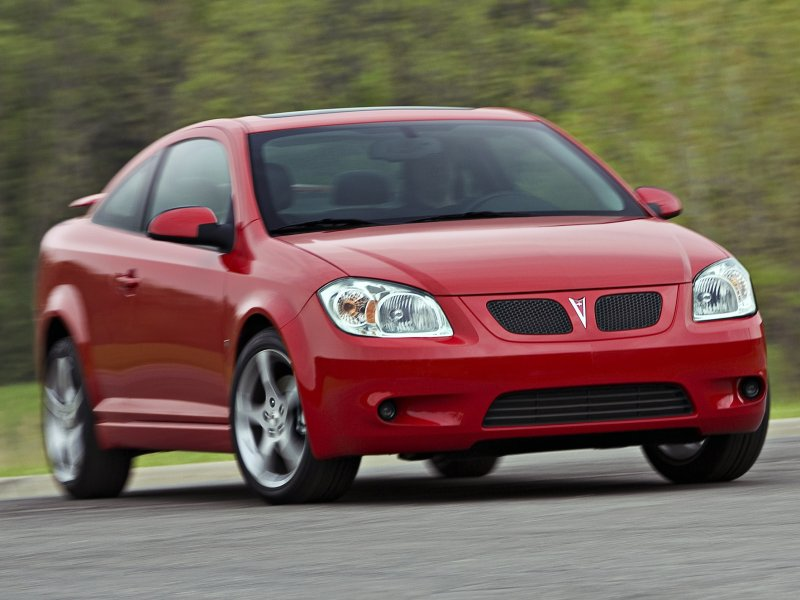
\includegraphics[scale=0.2]{\img/g5.png}
\quad
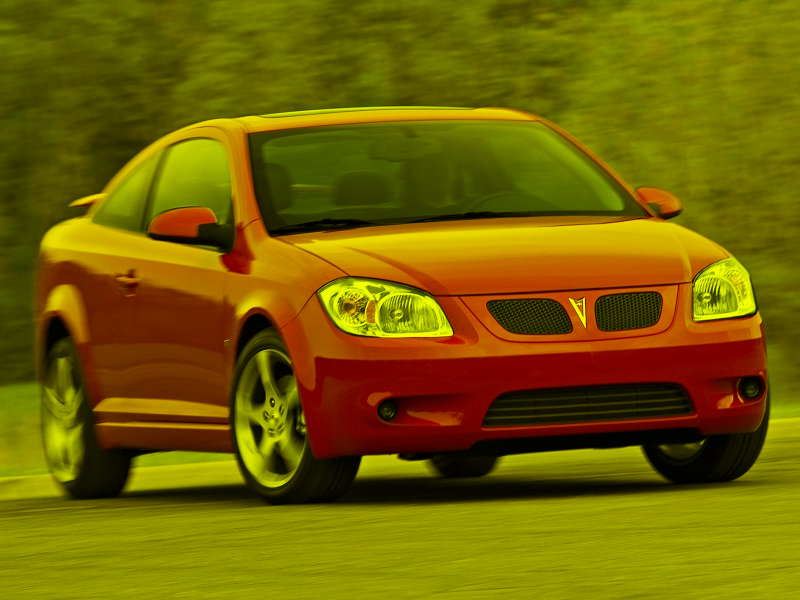
\includegraphics[scale=0.2]{\img/g5_remove-blue.png}
\end{center}
\caption{A sporty coupe before and after blue removal.}
\label{fig:g5_remove-blue}
\end{figure}

You should look at the file \lstinline'remove-blue.c0' to get an idea
of how this transformation works, and you should look at
\lstinline'README.txt' to see how to compile and run this
transformation against \lstinline'remove-blue-main.c0'.  You are
strongly encouraged to write some smaller test cases for your
programs. An example of what this should look like is given in
\lstinline'remove-blue-test.c0'.

Note that \lstinline'remove-blue.c0' doesn't use the \emph{pixel} or
\emph{imageutil} libraries. If \emph{your} code doesn't use the
\emph{pixel} or \emph{imageutil} libraries, you will fail style
grading!  While it is not required, you might want to try your hand at
modifying \lstinline'remove-blue.c0' to use the \emph{pixel} and
\emph{imageutil} libraries.


%% \begin{quote}
%% \begin{lstinline}[language={[coin]C}]
%% % cc0 -d imageutil.c0 quantize.c0 quantize-main.c0 -o quantize
%% % ./remove-blue -i \img/g5.png -q 6
%% \end{lstinline}
%% \end{quote}
%% Running this command should produce an image,
%% \lstinline'\img/g5_quantize.png', that is identical to the file
%% \lstinline'\img/g5-quantize6.png' distributed with the handout.



%% Try out the \lstinline'remove-blue'
%% transformation described in the ``Compiling and running'' instructions
%% above if you have not already done so; the code for this
%% transformation can be found at the end of the assignment.



%%% Local Variables:
%%% mode: latex
%%% TeX-master: "main"
%%% End:
